\documentclass[11pt,a4paper]{article}

\usepackage[margin=25mm]{geometry}
\usepackage{amsmath}
\usepackage{amssymb}
\usepackage{booktabs}
\usepackage{longtable}
\usepackage{graphicx}
\usepackage{xcolor}
\usepackage{enumitem}
\usepackage{fancyhdr}
\usepackage[hidelinks]{hyperref}

\definecolor{structcol}{HTML}{A83426}
\definecolor{seqcol}{HTML}{1F5891}
\definecolor{warncol}{HTML}{8A5710}

\pagestyle{fancy}
\fancyhf{}
\lhead{\small 3D-Chromatin-Aware Genomic FM}
\rhead{\small\thepage}
\renewcommand{\headrulewidth}{0.4pt}

\setlist{itemsep=2pt,parsep=0pt,topsep=4pt}

\newcommand{\code}[1]{\texttt{\small #1}}
\newcommand{\warn}[1]{\textcolor{warncol}{\textbf{#1}}}

\title{\vspace{-12mm}\textbf{Structure in the Recurrence}\\[2mm]
\large Conditioning Genomic Foundation Model Pretraining on 3D Chromatin Contacts}
\author{Project technical record}
\date{Compiled \today}

\begin{document}
\maketitle
\thispagestyle{fancy}

\begin{center}
\fcolorbox{structcol}{white}{\begin{minipage}{0.92\textwidth}
\small \textbf{No experimental results appear in this document.} No model has
been trained. The abstract is a proposal abstract. Every number reported comes
from a data-processing, parameter-accounting or unit-test script in the
repository, never from a training run. The working rule for this project is that
no figure reaches a draft unless it exists first in a logged output file.
\end{minipage}}
\end{center}

\vspace{4mm}

\section*{Abstract}
Genomic foundation models are pretrained on DNA sequence alone, yet much of the
regulatory logic they are asked to predict is carried by the genome's
three-dimensional folding, which determines which enhancers can reach which
promoters. Existing work combining sequence with chromatin contact data does so
after the sequence representation is already fixed: CHROME trains an encoder on
individual loci and only then adds a graph-attention layer over Hi-C contacts,
and Evo2HiC distils a frozen Evo~2 into a compact encoder using Hi-C as a
contrastive alignment target. In both, contact data shapes which learned
features are combined, never which features are learned. We propose instead to
place chromatin structure inside the pretraining computation. Contact-derived
features modulate the state-transition dynamics of a bidirectional Mamba
backbone, so Hi-C signal changes how far information propagates along the
sequence rather than only what each position encodes. The mechanism adds
$1.70\%$ to parameter count over a matched sequence-only baseline. We evaluate
whether a structure-shaped representation transfers---a question no
sequence-to-structure model has been asked, as a forward-citation sweep over 318
papers citing Akita and Orca confirms---using long-range regulatory and
variant-effect tasks together with a perturbation-sensitivity protocol on which
Evo~2 has been reported to fail. Controls include structure shuffled at
pretraining time and a distance-matched rewiring that tests whether any apparent
structural signal is genomic distance in disguise.

\vspace{2mm}
\noindent\textbf{Keywords:} genomic foundation models; 3D genome organisation;
Hi-C; topologically associating domains; state-space models; Mamba;
self-supervised pretraining; CTCF; variant effect prediction; representation
transfer.

\tableofcontents
\newpage

\section{The problem}

An enhancer can sit $10^5$ to $10^6$ base pairs from the promoter it regulates.
Nothing in the linear arrangement of the sequence explains how one reaches the
other. The genome resolves this by folding: a ring-shaped cohesin complex
extrudes a loop of DNA until it stalls at a pair of CTCF binding sites, and the
resulting loop places the enhancer physically against the promoter.

The stalling condition matters for what follows. Cohesin halts only when the two
CTCF motifs are \emph{convergent}---pointing toward each other. Motif presence is
insufficient; orientation decides. A sequence-only model sees the motif but
receives no training signal that makes orientation pairing across a
500\,kb gap consequential.

Three structures recur in the analysis. A \emph{topologically associating
domain} (TAD) is a region that contacts itself far more than its surroundings;
enhancers act almost exclusively within their own TAD, so boundaries determine
reachability. A \emph{loop} is a point-to-point contact between two anchors. An
\emph{A/B compartment} is a coarse partition into open, active and closed,
inactive regions.

\section{Related work and the gap}

\begin{longtable}{@{}p{4.6cm}ccp{3.4cm}c@{}}
\toprule
\textbf{Work} & \textbf{Seq.} & \textbf{Struct.} & \textbf{Structure enters at} & \textbf{Needed at inference} \\
\midrule
\endhead
HiCFoundation (2026) & no & yes & pretraining & yes \\
Hi-Cformer (2025) & no & yes & pretraining & yes \\
Evo~2 (2026) & yes & \textbf{no} & --- & no \\
Caduceus (2024) & yes & \textbf{no} & --- & no \\
GraphReg (2022) & feat. & yes & supervised, downstream & yes \\
CHROME (2026) & yes & yes & \textbf{stage 2, post-hoc} & \textbf{yes} \\
Akita / Orca & yes & target & supervised target & no \\
Evo2HiC (2025) & yes & yes & contrastive distillation & no \\
\midrule
\textbf{This project} & \textbf{yes} & \textbf{yes} & \textbf{self-supervised pretraining} & \textbf{target: no} \\
\bottomrule
\caption{Where 3D structure first influences the model. The bottom row is
unoccupied in the current literature.}
\end{longtable}

\subsection{The two nearest competitors}

\textbf{CHROME} (Ye et al., \emph{Briefings in Bioinformatics} 27(4):bbag360,
2026) filters Hi-C against a self-avoiding polymer null model simulated over
$5\times10^5$ chains, retaining $1.8$--$6\%$ of contacts, then runs two
graph-attention layers over signal-centred subgraphs with a 4\,Mb receptive
field at 5\,kb bins. Training has two stages: the encoder is trained on centre
nodes alone until validation saturates, and only afterwards are early layers
frozen and the graph module attached. Supervision is 751 ENCODE assays. Structure
never influences what the sequence encoder learns, and the contact graph is
required at inference.

\textbf{Evo2HiC} (Fang et al., bioRxiv 10.1101/2025.11.18.689171) distils a
frozen Evo~2 (7B) into a 3.6M-parameter CNN using two SigLIP contrastive
objectives, the second aligning the student to Hi-C patch embeddings. Structure
genuinely shapes a sequence encoder, but by aligning output embeddings, with no
objective over nucleotides. A keyword count over the full preprint returns zero
occurrences of \emph{ClinVar}, \emph{pathogenic}, \emph{eQTL}, \emph{variant},
\emph{masked}, \emph{MLM}, \emph{Mamba} and \emph{state space}. Their third
stated limitation is that they froze Evo~2 because fine-tuning it is
computationally hard, and that they intend to develop strategies for adapting it
with Hi-C data---this project's question, named as work they have not done.

\subsection{Two external findings that shaped the plan}

\textbf{Lee} (arXiv:2604.07196, April 2026) probed Evo~2 (7B) on 231 TAD boundary
regions and 120 convergent CTCF loops. Boundary deletions were penalised
\emph{less} than GC- and size-matched random controls (paired Wilcoxon
$p=0.405$); CTCF inversions and deletions likewise ($p=0.021$, $p=0.006$, in the
wrong direction). Generated loops reached median enrichment $0.054$ against a
reference of $0.388$. The paper concludes Evo~2 ``has learned local CTCF grammar
but misses higher-order 3D organization'' and prescribes bidirectional
architectures with explicit 3D contact inputs, citing Caduceus. This
substantially defuses failure mode F3 (Section~\ref{sec:failure}): if a
7B-parameter model with a 1M-token context cannot infer TAD-scale structure from
sequence, a 7.7M-parameter model will not either.

\textbf{DNALongBench} (\emph{Nature Communications} 16(1):10108, 2025) provides
five long-range tasks including enhancer--target interaction, eQTL and
contact-map prediction, already benchmarking Caduceus-Ph and Akita. Adopting it
for evaluation removes the objection that tasks were chosen to flatter.
Calibration: contact-map prediction is the hardest task in the suite, best
reported correlation $0.233$, by Akita.

\subsection{The negative result the contribution rests on}

A forward-citation sweep over 318 papers---118 citing Orca, 200 citing
Akita---found no work that takes either model's learned representations and
evaluates them on a task other than predicting folding. Their variant
applications all run the model twice, on reference and mutant sequence, and
compare predicted contact maps. Internal embeddings are never extracted, frozen
and probed, or fine-tuned into another head.

\section{Method}

\subsection{Baseline recurrence}

Per layer and direction, with channel index $i$ and state index $n$:
\begin{align}
(z, v) &= \mathrm{split}(W_{\text{in}} u_t) \\
x_t &= \mathrm{SiLU}(\mathrm{Conv1d}(v)_t) \\
(\delta'_t, B_t, C_t) &= \mathrm{split}(W_x x_t) \\
\Delta_t &= \mathrm{softplus}(W_{\delta} \delta'_t + b_{\delta}) > 0 \\
A_{i,n} &= -\exp(A^{\log}_{i,n}) < 0 \\
\bar{A}_{t,i,n} &= \exp(\Delta_{t,i} A_{i,n}) \in (0,1) \\
h_{t,i,n} &= \bar{A}_{t,i,n}\, h_{t-1,i,n} + \Delta_{t,i} B_{t,n} x_{t,i} \\
y_{t,i} &= \textstyle\sum_n C_{t,n} h_{t,i,n} + D_i x_{t,i}
\end{align}

\subsection{The structural modification}

Let $s_t \in \mathbb{R}^{d_s}$ be the structural context at position $t$, derived
from Hi-C. Two terms are added:
\begin{align}
\Delta_t &= \mathrm{softplus}\big(W_{\delta}\delta'_t + b_{\delta}
              + \textcolor{structcol}{W_{\Delta s} s_t}\big) \\
p_t &= \mathrm{softplus}\big(\textcolor{structcol}{w_g^{\top} s_t + b_g}\big) \ \geq 0 \\
\bar{A}_{t,i,n} &= \exp\big(\Delta_{t,i} A_{i,n} \textcolor{structcol}{- p_t}\big)
\end{align}

The first retunes the memory length of each channel. The second is a
non-negative damping that only shortens memory: at a TAD boundary the model can
raise it and cut the state.

\paragraph{Why this is not an input feature.} Appending $s_t$ to the input would
reach only $\bar{B}_t x_t$, the term governing how much of the current token
enters. It cannot alter $\bar{A}_t$, which governs what survives. Because
$\Delta$ enters $\bar{A}$ inside an exponential, structure here sets the
effective memory horizon
\begin{equation}
\tau_{t,i} = \frac{-1}{\Delta_{t,i} A_{i,n} - p_t} \quad \text{(tokens)},
\end{equation}
that is, how \emph{far} information travels rather than what is encoded. This is
the class of constraint that contrastive alignment on output embeddings cannot
express, and it is the entire novelty claim.

\paragraph{Relationship to hard state resets.} As $p_t \to \infty$,
$\bar{A}_t \to 0$ and $h_t = \bar{B}_t x_t$: a hard reset. The mechanism is the
soft, learned relaxation of TAD-conditioned state resetting, which is recorded as
future work.

\paragraph{Initialisation.} $W_{\Delta s} = 0$, $w_g = 0$, $b_g = -4$. The model
is then numerically indistinguishable from the baseline at step zero, so any
divergence is attributable to learned structural signal. Zero initialisation of
$W_{\Delta s}$ does not block learning, since
$\partial L/\partial W_{\Delta s} = (\partial L/\partial \Delta)\, s_t^{\top}$.

\subsection{Parameter accounting}

Computed by instantiating both models and summing parameter tensors
(\code{scripts/param\_accounting.py}, \code{scripts/test\_model.py}).

\begin{table}[h]\centering
\begin{tabular}{@{}lrrr@{}}
\toprule
Configuration & Total & Added & $\Delta$ \\
\midrule
Sequence-only baseline & 7{,}725{,}312 & --- & --- \\
$d_s=2$, with encoder & 7{,}758{,}354 & 33{,}042 & $+0.428\%$ \\
$d_s=8$, with encoder & 7{,}856{,}952 & 131{,}640 & $+1.704\%$ \\
$d_s=8$, \textbf{no encoder} (recommended) & 7{,}856{,}672 & 131{,}360 & $+1.700\%$ \\
\bottomrule
\end{tabular}
\caption{All configurations sit inside the 5\% matched-parameter budget.}
\end{table}

\section{Implementation}

\subsection{Scan backends}

The selective scan has two implementations, selected by device.

The reference implementation is a sequential loop over positions: correct,
differentiable, and what the CPU unit tests run at small $L$. It is not viable at
$L=32{,}768$, which would require $32{,}768 \times 16 \times 2$ Python iterations
per forward pass.

Production requires a fused kernel, and the two structural terms differ sharply
in how they cooperate with the stock one. \textbf{The $\Delta$ bias is free}:
\code{mamba\_ssm}'s \code{selective\_scan\_fn} takes \code{delta} as an argument,
so the bias is added before the call. \textbf{The permeability term $p_t$ is
not expressible} through that interface: it needs
$\bar{A} = \exp(\Delta A - p)$, and folding $p$ into $\Delta$ would require
$\Delta' = \Delta + \log(g)/A_{n}$, which depends on the state index $n$. A
single per-channel $\Delta$ cannot produce a decay uniform across $n$.

A custom Triton kernel was therefore written
(\code{src/chromfm/scan\_triton.py}), carrying $p$ through both forward and
backward. It uses one program per (batch, channel) pair, checkpoints the state at
chunk boundaries, and in the backward replays each chunk from its checkpoint
before running the adjoint recurrence, keeping memory at
$O(BD\,\tfrac{L}{\text{chunk}}N)$ rather than $O(BDLN)$.

\begin{center}
\fcolorbox{warncol}{white}{\begin{minipage}{0.92\textwidth}
\small \warn{The Triton kernel has never been executed.} It was written on a
CPU-only machine with no CUDA device and no Triton install. The recurrence and
its adjoint were derived by hand and the code is syntactically complete, but
nothing is numerically confirmed. \code{scripts/validate\_kernel.py} must be run
on the GPU box before any training. A scan with a subtly wrong gradient produces
a smooth, plausible loss curve while training the wrong model.
\end{minipage}}
\end{center}

Both arms must use the same backend, or the matched-compute comparison is
confounded. The baseline therefore runs on this scan too, even though it never
supplies $p$.

\subsection{Dataset layer}

\begin{table}[h]\centering
\begin{tabular}{@{}lr@{}}
\toprule
Window & 32{,}768 bp \\
Train stride & 16{,}384 (50\% overlap) \\
Evaluation stride & 32{,}768 (no overlap) \\
Train windows & 5{,}422 \\
Validation windows & 273 \quad (chr9:120{,}029{,}184--128{,}974{,}848) \\
Test windows & 242 \quad (chr9:130{,}023{,}424--137{,}953{,}280) \\
Dropped & 1{,}054 on N fraction, 799 on structural coverage, 126 buffer \\
\bottomrule
\end{tabular}
\caption{Window index. Verified: zero training windows touch either held-out
region; both evaluation splits are fully contained with no internal overlap.}
\end{table}

Window length follows from the memory-horizon measurement rather than
convention: the 16-layer relayed horizon is roughly 16{,}000 tokens, so 32{,}768
already exceeds what the stack can span.

Three policies are implemented in the dataset builder rather than in either
training script, so the two arms cannot diverge on them:

\begin{enumerate}[label=(\roman*)]
\item \textbf{$\phi$ is interpolated, not stepped.} Linear interpolation between
bin centres. Measured inside one window, a step function yields 7 distinct values
per feature; interpolation yields 32{,}757. Seven values across a window is the
precondition for failure mode F4.
\item \textbf{N has its own token and a budget.} 12.00\% of chr9 is unresolved;
windows above 10\% N are dropped.
\item \textbf{Invalid bins are masked, never NaN.} A position is structurally
valid only when both flanking bins are usable. Invalid positions receive
$\phi=0$, the standardised mean, plus a validity flag. A NaN reaching
$W_{\Delta s}s_t$ would poison the entire recurrence.
\end{enumerate}

Reverse-complement augmentation reverses and complements the tokens, then
reverses $\phi$ and negates its two antisymmetric coordinates
(\code{directionality\_2Mb}, \code{upstream\_mass\_frac}).

\section{Pilot data}

\subsection{Provenance}

Source is 4D Nucleome experiment set \textbf{4DNES3JX38V5}: in situ Hi-C on
GM12878, MboI with bio-dATP, Lieberman Aiden lab, published as Rao et al.\ 2014
(PMID 25497547), aligned to GRCh38. The multi-resolution contact matrix
(4DNFIXP4QG5B) is 27.4\,GB and is never downloaded; the pipeline reads a
near-diagonal band directly over HTTP range requests in six and a half minutes.
Boundary calls, insulation and compartment tracks are mirrored as independent
validation targets, not as model inputs. Sequence is Ensembl release 113;
annotation is GENCODE release 47.

\subsection{Measured properties}

\begin{table}[h]\centering
\begin{tabular}{@{}lr@{}}
\toprule
chr9 length, from the contact matrix & 138{,}394{,}717 bp \\
chr9 length, from the Ensembl FASTA & 138{,}394{,}717 bp \\
Bins at 5\,kb & 27{,}679 \\
Band entries retained & 7{,}108{,}483 \\
Band occupancy & 0.6451 \\
Bins with no balancing weight & 19.31\% \\
Unresolved sequence (N) & 12.00\% \\
Bins with a complete feature vector & 21{,}519 \ (77.74\%) \\
\bottomrule
\end{tabular}
\end{table}

The two identical lengths are the first coordinate-alignment check. A second,
stronger one emerged unplanned: the pipeline returned nothing for chr9 between 48
and 58\,Mb. That is the centromere and the 9q12 heterochromatic block, which
GRCh38 represents as a gap. The sequence file is 100\% unresolved from
approximately 46 to 60\,Mb, and the contact matrix has no usable bins from 43.27
to 60.52\,Mb. Two files from different institutions placing the same feature at
the same coordinates is stronger evidence than a matching chromosome length.

\subsection{Structural features}

\begin{table}[h]\centering
\begin{tabular}{@{}clll@{}}
\toprule
Index & Feature & Window & Under reverse complement \\
\midrule
0--2 & insulation score & 100, 250, 500\,kb & symmetric \\
3 & directionality index & 2\,Mb & \textbf{antisymmetric} \\
4 & log contact density & 2\,Mb & symmetric \\
5 & upstream mass fraction & 2\,Mb & \textbf{antisymmetric} \\
6 & short-to-long range ratio & 100\,kb / 2\,Mb & symmetric \\
7 & A/B compartment eigenvector & 250\,kb, GC-oriented & symmetric \\
\bottomrule
\end{tabular}
\caption{The symmetry column is load-bearing: failure mode F7 is the case where
features 3 and 5 cancel between the forward and reverse passes.}
\end{table}

\subsection{Validation against independent tracks}

\begin{table}[h]\centering
\begin{tabular}{@{}llr@{}}
\toprule
Our feature & Against 4DN's own track & Pearson $r$ \\
\midrule
Insulation, 100\,kb window & 4DNFIBMOGOZC & $+0.9969$ \\
Insulation, 250\,kb window & 4DNFIBMOGOZC & $+0.7802$ \\
Insulation, 500\,kb window & 4DNFIBMOGOZC & $+0.4895$ \\
A/B compartment eigenvector & 4DNFILYQ1PAY & $+0.9759$ \\
\bottomrule
\end{tabular}
\caption{The 100\,kb window reproduces 4DN's track almost exactly, identifying
their diamond window and confirming the implementation. Declining correlation at
larger windows is the expected consequence of comparing different window sizes
against a fixed reference.}
\end{table}

A TAD and a loop are both visible in the processed data. The loop lies at
chr9:136{,}485{,}000 paired with 136{,}625{,}000, 140\,kb apart, at 7.5 times its
distance-matched expectation, with six CTCF ChIA-PET read pairs from an
independent assay at the same anchors. Its upstream anchor falls on
\emph{NOTCH1} (chr9:136{,}494{,}433--136{,}546{,}048).

\begin{figure}[htbp]\centering
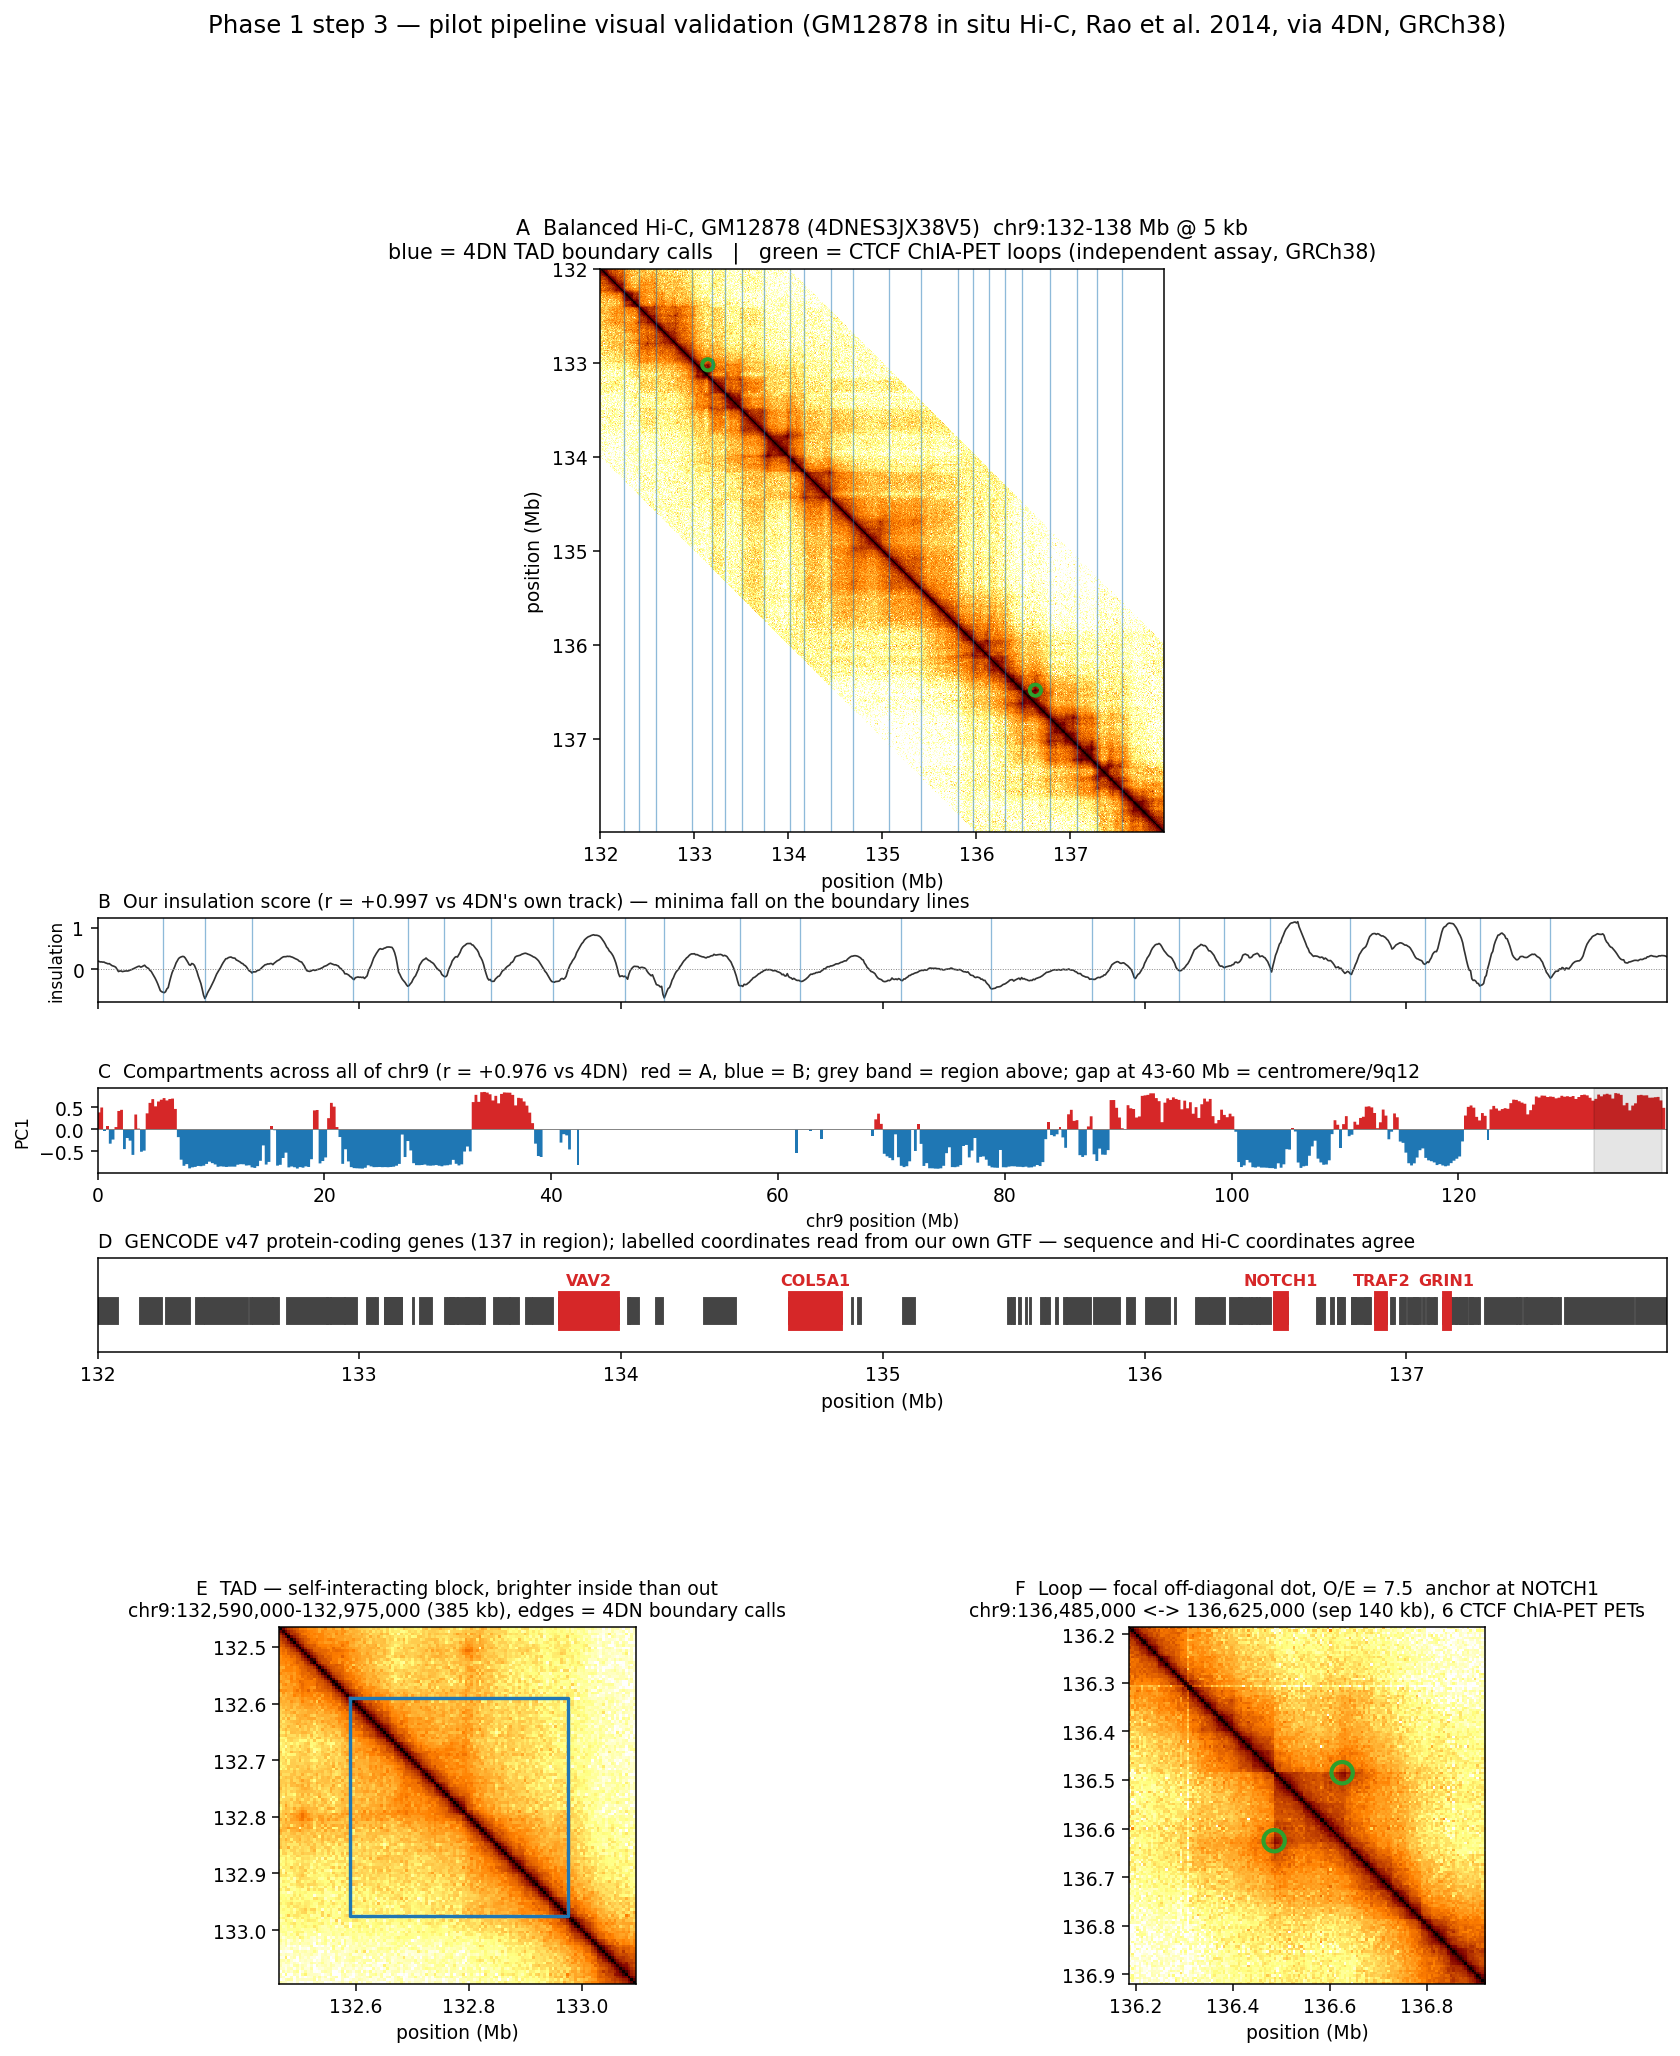
\includegraphics[width=\textwidth]{../figures/phase1_validation.png}
\caption{Pilot pipeline validation. (A) Balanced contacts with 4DN boundary calls
in blue and CTCF ChIA-PET loops in green. (B) Our insulation score. (C)
Compartments across all of chr9; the blank interval at 43--60\,Mb is the
centromere. (D) GENCODE genes with coordinates read from our own annotation.
(E) A 385\,kb TAD. (F) The NOTCH1-anchored loop.}
\end{figure}

\section{Failure modes and controls}
\label{sec:failure}

\subsection{Shuffled-structure controls}

\begin{longtable}{@{}clp{4.0cm}p{4.4cm}@{}}
\toprule
ID & Control & Destroys & Rules out \\
\midrule
\endhead
S0 & zero the signal & everything & establishes the sequence-only floor at identical parameter count \\
S1 & permute across bins & alignment and autocorrelation & primary reliance probe \\
S2 & circular shift, 10\,Mb & alignment only & ``any smooth auxiliary channel would do'' \\
S3 & distance-matched rewire & locus-specific structure & \textbf{``structure is genomic distance in disguise''} \\
\bottomrule
\caption{S3 is the control that can end the project.}
\end{longtable}

Contact probability falls smoothly with genomic distance. If a model performs as
well on distance-matched fake structure as on real structure, what it learned is
a re-parameterised positional prior and the central claim is false however good
the headline number looks.

The gate passes only if degradation under shuffling is positive with a 95\%
bootstrap confidence interval excluding zero \emph{and} is at least twice the
across-seed standard deviation of the real-structure runs. Significance alone is
insufficient; the effect-size floor prevents a $p$-value standing in for an
effect.

\subsection{The eight failure modes}

\begin{longtable}{@{}clp{4.4cm}p{4.6cm}@{}}
\toprule
& Failure & Symptom & Status \\
\midrule
\endhead
F1 & bias absorbed into $b_\delta$ & trains to baseline loss & highest probability; mitigated by genome-wide standardisation \\
F2 & softplus saturation & structural weights never move & \textbf{observed}; $b_g$ changed $-8 \to -4$ \\
F3 & structure inferable from sequence & structural input redundant & \textbf{largely defused} by Lee's Evo~2 probe \\
F4 & bin longer than memory horizon & trains to baseline loss & \textbf{precondition confirmed}; mitigated by interpolation \\
F5 & permeability gate stays at zero & half the mechanism inert & monitor the distribution of $p$ \\
F6 & gradient starvation & structural pathway never learns & 1.7\% of parameters behind two nonlinearities \\
F7 & forward and reverse cancel & trains to baseline loss & two of eight features flip sign under RC \\
F8 & structural encoder collapses & reduces to F1 & \textbf{eliminated} if the encoder is removed \\
\bottomrule
\end{longtable}

F1, F4 and F7 produce the same symptom: the model trains to baseline performance
and raises no error. Four diagnostics therefore run continuously---the variance
the structural pathway contributes to the timescale, the distribution of the
permeability penalty, the growth of the structural weight norm, and a probe
asking whether the baseline model's hidden states already predict the structural
signal.

\subsection{Memory horizon, measured}

At the reference initialisation, horizons run from 0.6 tokens at the fast end to
994 at the slowest, median 14.9. A 5\,kb bin is 5{,}000 tokens, so no
channel-state pair spans a single bin; $\tau_{\max}/\text{bin} = 0.199$. Sixteen
layers relaying extends reach to roughly 15{,}900 tokens, still short of a
385\,kb TAD.

$\Delta$ is learned and can grow, so this is not proof of failure. It constrains
the sequence-only baseline exactly as much as the structural model, which raises
a question worth settling before spending GPU time: can a model of this size
represent TAD-scale dependencies at all? \textbf{Phase 3 must therefore report
the trained memory horizon, and that measurement gates Phase 4.}

\section{Decisions of record}

\begin{longtable}{@{}clp{4.2cm}p{5.2cm}@{}}
\toprule
& Decision & Choice & Reasoning \\
\midrule
\endhead
1 & Mechanism & structural bias in the recurrence & unreachable by contrastive alignment on output embeddings; contains hard state resets as its limit; cheap to falsify \\
2 & Reverse complement & Caduceus-PH (augmentation) & equivariance is orthogonal to the hypothesis; coupling them makes a null result uninterpretable \\
3 & Hi-C resolution & 5\,kb, 1\,kb as ablation & comparability with CHROME; both levels are in the same file \\
4 & Cross-species scope & out for this paper & Evo2HiC uses 177 species, HiCFoundation 316; entering that lane splits compute against better-resourced groups \\
5 & Permeability term & \textbf{keep}, via custom kernel & retains the soft-reset semantics and the link to future work \\
\bottomrule
\end{longtable}

\section{Change log}

Every substantive change to the project is recorded here with its reason.

\subsection*{2026-08-10}

First session on the L40S box. Environment built, pipeline reproduced from a
clean tree, custom kernel executed for the first time. No model trained.

\begin{itemize}
\item \textbf{Environment.} \code{torch 2.6.0+cu124}, \code{triton 3.2.0},
Python 3.10, venv \code{3d-gen/} (added to \code{.gitignore}).
\code{torch.cuda.device\_count() = 2}; both devices report NVIDIA L40S,
compute capability 8.9, 44.4\,GiB.
\item \warn{NVML is broken on this box and \code{nvidia-smi} does not run.}
The loaded kernel module is 580.126.09 while the userspace libraries are
580.173.02. CUDA is unaffected---\code{cuInit} returns 0, both devices
enumerate and compute---but NVML-based utilisation and temperature logging is
unavailable until the modules are reloaded, which needs root. Recorded because
the run config is supposed to carry the driver version, and the number
\code{nvidia-smi} would have reported cannot be obtained here.
\item \textbf{Pipeline reproduced exactly from a clean tree.}
\code{phase1\_acquire.py} assembled \textbf{7{,}108{,}483} unique
upper-triangle band entries with all three auxiliary md5s verified;
\code{phase1\_features.py} reproduced insulation $r=+0.9969$ ($n=21{,}740$) and
compartments $r=+0.9759$ ($n=22{,}250$) against 4DN's own tracks, with
21{,}519/27{,}679 bins carrying a complete $\phi$; \code{phase1\_dataset.py}
built \textbf{5{,}422 / 273 / 242} train/val/test windows with drop counts
1{,}054 (N fraction), 799 (structural coverage), 126 (buffer), 2 (short).
Every one of these matches \code{docs/data\_card.md} exactly, so the data
layer is confirmed reproducible on a second machine rather than only on the
machine that built it.
\item \warn{\code{data/pilot\_manifest.json} now differs from the committed
copy, and none of the differences are content.} The committed manifest was
written on Windows. Rebuilding on Linux changed (i) path separators,
\code{data\textbackslash raw\textbackslash} to \code{data/raw/}; (ii) the byte
size of the two text files, because the Windows copies had CRLF line endings
---\code{chr9.fa} shrank by exactly 2{,}306{,}580 bytes against 2{,}306{,}580
lines, and the GTF by exactly 169{,}673 bytes against 169{,}673 lines, one
byte per line in each case; and (iii) the md5 of the two \code{.npz} files,
whose byte sizes are nevertheless \emph{identical}, because a zip central
directory records the creating platform---\code{create\_system} is 3 (Unix)
here and 0 (Windows) there. The md5s of the three files downloaded from 4DN,
which are the ones checked against the 4DN API, are unchanged. Band contents
re-verified directly: 7{,}108{,}483 entries, 0 non-finite, min
$4.25\times10^{-6}$ / median $3.10\times10^{-4}$ / max 0.942, 27{,}679 bins,
5{,}345 (19.31\%) without a balancing weight---every figure matching
\code{docs/data\_card.md} §4. Whether to commit the Linux manifest is a
judgement call left to the PI; a manifest whose md5s are platform-dependent
cannot serve as a cross-platform integrity check for the derived files, only
for the downloaded ones.
\item \textbf{\code{test\_model.py}: 16/16 passed} on this box, unchanged.
\item \textbf{Triton kernel executed for the first time and validated:
34/34 checks passed} (\code{validate\_kernel.py}, exit 0) across no-$p$,
with-$p$, multi-chunk and ragged-final-chunk configurations, including the
assertion that $\partial L/\partial p \neq 0$.
\item \textbf{Three kernel defects fixed, all in the Triton lowering rather
than the mathematics.} The hand-derived adjoint was correct as written.
(i) \code{CHUNK} was a module-level global, which Triton refuses to read from
a \code{@jit} function; it is now a \code{tl.constexpr} kernel parameter.
(ii) The chunk walk used \code{range(NCHUNK-1,-1,-1)}; Triton lowers
\code{range} to \code{scf.for}, which requires a non-negative step, so both
reversed loops now count up and invert the index by hand.
(iii) The inner loops used \code{tl.minimum(CHUNK, L-t0)} as a trip count;
they now always run \code{CHUNK} times and predicate on $t<L$.
\item \warn{The backward is not bitwise reproducible.} \code{dBmat},
\code{dCmat} and \code{dp} are accumulated with \code{tl.atomic\_add} across
the $d_{\text{inner}}$ programs, so their summation order varies between runs.
Measured relative spread over five repeats at $B=2$, $D=512$, $L=512$:
$1.0\times10^{-6}$, $9.6\times10^{-7}$ and $8.9\times10^{-7}$ respectively;
\code{du}, \code{ddelta}, \code{dA} and \code{dDskip} were bitwise identical.
This is fp32 rounding noise, not a defect, but it means seed-identical runs
reproduce to fp32 tolerance and not to the bit. The paper must not claim
bit-exact reproducibility.
\item \textbf{Kernel checked beyond the supplied harness}, which runs at
$D=64$. Added checks at the real width $d_{\text{inner}}=512$, at 64 chunks,
and at $L=1$ and $L=65$; all agree with the reference. Width matters because
the cross-channel atomics only contend at width.
\item \textbf{Scan checkpoint memory measured}, since it bounds the Phase 3
batch size: 16.0\,MiB per sample per scan at $d_{\text{inner}}=512$,
$d_{\text{state}}=16$, $L=32{,}768$, which is 0.50\,GiB per sample across 16
layers and 2 directions, or 4.0\,GiB at batch 8 before any other activation.
\item \textbf{TeX Live installed user-local} (TinyTeX). The box had no LaTeX
engine and no root, so \code{build\_project\_doc.py} could not run at all.
\end{itemize}

\subsection*{2026-08-10 (second entry) --- Phase 3 training harness}

\code{scripts/train.py} written. Results are recorded in a later entry; this one
covers the harness and the platform findings only.

\begin{itemize}
\item \warn{NCCL cannot be used on this box.} It calls \code{nvmlInit\_v2()}
during topology discovery, which fails for the same driver mismatch that breaks
\code{nvidia-smi}. \code{init\_process\_group("nccl")} is lazy and succeeds
anyway, so the failure surfaces at the first collective inside DDP's
constructor. The script therefore probes NVML directly and falls back to
\textbf{gloo}. Measured cost of the fallback: none detectable---two GPUs give
$2.00\times$ the single-GPU throughput (0.756 windows/s on one L40S,
1.51 windows/s on two).
\item \warn{PyTorch's CUDA caching allocator also calls NVML} when it reports
memory pressure, so an out-of-memory condition surfaces as
\code{INTERNAL ASSERT FAILED ... nvmlInit\_v2\_} rather than as
\code{CUDA out of memory}. Anyone reading that traceback later should read it
as OOM.
\item \textbf{Kernel made 1.42$\times$ faster, and re-validated.} The scan's
state vector is $d_{\text{state}}=16$ elements wide, so Triton's default
\code{num\_warps=4} gave each program 128 lanes for 16 lanes of work. Setting
\code{num\_warps=1} took the real config from 7.55 to 5.30\,s/step. Per-step
losses were identical to the default across the benchmark, and
\code{validate\_kernel.py} was re-run afterwards: 34/34.
\item \textbf{Gradient checkpointing implemented and then measured not to
help.} The hypothesis was that the scan is latency-bound and a bigger batch
bought with recompute would be nearly free. Batch scaling turned out to be
linear---the GPU is already saturated at batch 2---so checkpointing costs its
recompute undiluted: 1.32\,s/window at batch 2 without it against
1.49\,s/window at batch 8 with it. The code is retained behind
\code{--grad-checkpoint}, off by default, as the lever to reach for if
$d_{\text{model}}$ or the window grows.
\item \textbf{fp32 throughout, no autocast}, because the scan was validated in
fp32 only. Training the experiment in bf16 would put it back on an unvalidated
numeric path through a hand-written recurrence.
\item \textbf{The baseline runs the custom Triton scan} even though it never
supplies $p$, so the matched-compute claim against the structural arm is real
rather than nominal.
\item \textbf{N is excluded from masking and from the loss.} 12.00\% of chr9 is
N and a window may carry up to 10\%. Including N would deflate
bits/nucleotide by an amount that varies with each window's N content. The
reported metric is therefore bits per \emph{resolved} nucleotide, and its
uniform-random floor is exactly 2.000 bits.
\item \warn{$\tau$ is measured two ways and they are not interchangeable.}
\code{BiMambaLM.tau\_stats()} derives $\tau$ from \code{dt\_proj.bias} alone.
That is a fair proxy at initialisation, where \code{dt\_proj.weight} is small,
but after training $\Delta$ is dominated by the input-dependent term
$W_{dt}\delta'_t$, and a bias-only $\tau$ can be badly wrong. The script logs
\code{tau\_stats()} because the runbook asks for it, and separately measures
\emph{empirical} $\tau$ from the $\Delta$ actually produced on validation
batches. \textbf{The F4 gate must be read off the empirical numbers.}
\item \textbf{\code{num\_workers} defaults to 0.} \code{WindowDataset} owns an
\code{np.random.default\_rng} for reverse-complement augmentation; under
multiple loader workers each worker copies it, so the augmentation stream would
depend on how the sampler sharded and seeds would stop being reproducible.
\end{itemize}

\subsection*{2026-08-07}

\begin{itemize}
\item \textbf{Phase 0 completed.} Eleven papers mapped. Two competitors found
that were not on the original reading list: Evo2HiC, which is closer to the
thesis than CHROME, and Lee's Evo~2 probe, which supports it.
\item \textbf{Differentiator retired.} ``Structure at training, sequence-only at
inference'' was dropped as a claim against Evo2HiC, whose DNA-only encoder has
the same property. It still holds against CHROME.
\item \textbf{Forward-citation sweep.} 318 papers checked; no work probes Akita
or Orca representations on a non-folding task. The transfer gap stands.
\item \textbf{Mechanism (a) selected}; (b) and (c) documented but not pursued.
\item \textbf{Memory horizon measured.} $\tau_{\max} = 994$ tokens against a
5{,}000-token bin. Consequence: $\phi$ interpolation became mandatory, and a
trained-$\tau$ measurement was added as a Phase 4 gate.
\item \textbf{Pilot acquired and validated.} Insulation $r=+0.9969$ and
compartments $r=+0.9759$ against independent 4DN tracks. A TAD and a
ChIA-PET-corroborated loop confirmed visually.
\item \textbf{Three assembly traps caught.} A 1{,}425\,kb ``loop'' that was
sparse-corner noise; an hg19 \emph{ABL1} coordinate used to choose a GRCh38
region; and the standard GEO loop list for this dataset, which is hg19---detected
because its largest chr9 anchor exceeds the length of GRCh38 chr9.
\item \textbf{Dataset layer built.} Splits verified exact after a first version
allowed held-out windows to straddle their region edge.
\item \textbf{Model implemented; two bugs found by unit tests.} The
reverse-complement sign flip was being applied to the encoded signal rather than
to raw $\phi$, where the encoder has already mixed all eight coordinates,
making the operation meaningless. Separately, $A$ was broadcast by trailing-axis
alignment, which matches the state dimension against sequence length and only
agrees when $L = d_{\text{inner}}$; the first test passed only because it used
$L=64$ with $d_{\text{inner}}=64$.
\item \textbf{$b_g$ changed from $-8$ to $-4$.} The gradient through softplus is
$\sigma(b_g)$, so $-8$ attenuated the gate's learning signal roughly
3000-fold---failure mode F2, self-inflicted by our own initialisation. Measured
effect on the gate gradient: $2.06\times10^{-7} \to 7.69\times10^{-6}$.
\item \textbf{Encoder bottleneck identified.} $\partial L/\partial s =
W_{\Delta s}^{\top}\partial L/\partial \Delta$ with $W_{\Delta s}$
zero-initialised, so the encoder receives exactly zero gradient on step zero and
roughly $10^{-9}$ afterwards against $10^{-4}$ for the matrix in front of it.
Recommendation: remove the encoder and feed the eight standardised features
directly at $d_s=8$, costing $+1.700\%$ parameters and eliminating F8.
\item \textbf{Triton kernel written} for the permeability term, with a GPU
validation harness. Unverified until executed.
\end{itemize}

\section{Open items}

\begin{itemize}
\item \textbf{Decide whether bit-exact reproducibility is required.} If it is,
the atomics in the backward must be replaced with a deterministic reduction,
at a performance cost. If it is not---the reasonable reading, given that the
Phase 5 gate is across-seed variance rather than a single number---say so
explicitly, because the spread is measured and small.
\item \textbf{Restore \code{nvidia-smi}} by reloading the NVIDIA kernel
modules, or accept that no driver-level utilisation figure can be logged
alongside the runs.
\item \textbf{Confirm the encoder removal} ($d_s=8$, no encoder), which changes
parameter figures recorded in three documents.
\item \textbf{Read CHROME line by line.} The summary here came from automated
extraction of the PMC full text.
\item \textbf{Obtain Orca's Results section}, paywalled at \emph{Nature
Genetics} with no PubMed Central deposit. The claim that its representations were
never evaluated on a non-folding task rests on the abstract, all ten
extended-data captions and the section headings, not the body.
\item \textbf{Re-check Evo2HiC} for a revision adding variant evaluation before
Phase 4 commits GPU time; that would close the one contribution nothing
currently contests.
\item \textbf{Re-check Lee's preprint} for peer-review status before it carries
weight in a methods section.
\end{itemize}

\section{What happens next}

Phase 3 trains the sequence-only baseline, logging every hyperparameter, seed and
metric before any structural model exists, so no flattering comparison can be
selected after the fact. That run must also report the trained memory horizon,
which decides whether a model of this size can represent TAD-scale dependencies
at all. If it cannot, the mechanism is re-scoped to sub-TAD structure or the
model is enlarged, and that decision is taken before Phase 4 rather than after.

\vspace{6mm}
\hrule
\vspace{2mm}
\noindent\small Every measured number in this document traces to a named script:
\code{phase1\_acquire.py}, \code{phase1\_features.py},
\code{phase1\_validate\_visual.py}, \code{phase1\_dataset.py},
\code{param\_accounting.py}, \code{f4\_memory\_horizon.py},
\code{test\_model.py}. Literature claims are sourced in
\code{docs/related\_work.md}; the mechanism is specified in
\code{docs/architecture\_spec.md}; data provenance is in
\code{docs/data\_card.md}.

\end{document}
